\documentclass[a4paper,14pt]{article}
\usepackage[left=2cm,right=2cm, top=2cm,bottom=2cm, bindingoffset=0cm]{geometry}
\usepackage[T2A]{fontenc}
\usepackage[utf8]{inputenc}
\usepackage[english,russian]{babel}
\usepackage{amsmath,amsfonts,amssymb,amsthm,mathtools,graphicx}
\usepackage{fancybox,fancyhdr}
\usepackage{tabularx}
\usepackage{multirow}
\usepackage{bigstrut}
\usepackage{booktabs}
\usepackage{float}
\usepackage{xcolor}
\usepackage{array}
\usepackage{caption}

\graphicspath{{./}}
\DeclareGraphicsExtensions{.pdf,.png,.jpg}

\author{Ануфриев Андрей}

\date{\today}

\begin{document}

    \begin{figure}[h]
        \centering
        \begin{minipage}{0.45\linewidth}
            \centering
            
\includegraphics[width=\linewidth]{slogan_chernyy}
            \label{fig:slogan}
        \end{minipage}
        \hfill
        \begin{minipage}{0.45\linewidth}
            \centering
            
\includegraphics[width=\linewidth]{cs-logo}
            \label{fig:logo}
        \end{minipage}
    \end{figure}
    \begin{table}[htbp]
        \centering
        \begin{tabular}{lrlr}
            Группа & \qquad \qquad P3219 & К работе допущен & \qquad \qquad \qquad \qquad \qquad \qquad \\
            \cmidrule{2-2}\cmidrule{4-4}
            Студент &  \qquad \qquad Ануфриев А.С.  & Работа выполнена & \qquad \qquad \qquad \qquad \qquad \qquad \\
            \cmidrule{2-2}\cmidrule{4-4}
            Преподаватель & \qquad \qquad Коробков М.П. & Отчет принят & \qquad \qquad \qquad \qquad \qquad \qquad \\
            \cmidrule{2-2}\cmidrule{4-4}
        \end{tabular}%
    \end{table}%
    \vspace{2cm}
    \begin{center}
        \LARGE
        Отчет по лабораторной работе № 3.05 \\
        Определение ширины запрещённой зоны полупроводника и температурного коэффициента сопротивления металла

    \end{center}
    \vspace{13cm}
    \begin{center}
        2026 год
    \end{center}
    \newpage

% ===== ЦЕЛИ =====
\section{Цели работы}
\begin{enumerate}
    \item Получить зависимость электрического сопротивления металлического и полупроводникового образцов в диапазоне температур от комнатной до $75\,^{\circ}\mathrm{C}$.
    \item По результатам п.\,1 вычислить температурный коэффициент сопротивления металла и ширину запрещённой зоны полупроводника.
\end{enumerate}

% ===== РАБОЧИЕ ФОРМУЛЫ =====
\section{Рабочие формулы и теоретические сведения}

\subsection*{Металл}

Сопротивление металла линейно зависит от температуры:
\begin{equation}
    R_\text{м} = R_0\,(1 + \alpha\, t),
    \label{eq:metal}
\end{equation}
где $R_0$ — сопротивление при $0\,^{\circ}\mathrm{C}$, $\alpha$ — температурный коэффициент сопротивления (ТКС), $t$ — температура в градусах Цельсия.

Сопротивление образца вычисляется из закона Ома:
\begin{equation}
    R = \frac{U}{I}.
    \label{eq:ohm}
\end{equation}

Для нахождения $\alpha$ методом пар из системы уравнений (\ref{eq:metal}) для двух точек $i$ и $j$:
\begin{equation}
    \alpha_{ij} = \frac{R_i - R_j}{R_j\,t_i - R_i\,t_j}.
    \label{eq:alpha_pair}
\end{equation}

\subsection*{Полупроводник}

Сопротивление собственного полупроводника зависит от температуры экспоненциально:
\begin{equation}
    R_\text{п} = R_m\,\exp\!\left(\frac{E_g}{2kT}\right),
    \label{eq:semi}
\end{equation}
где $E_g$ — ширина запрещённой зоны, $k = 1{,}38065\times10^{-23}$\,Дж/К — постоянная Больцмана, $T$ — абсолютная температура.

Логарифмирование даёт линейную зависимость:
\begin{equation}
    \ln R_\text{п} = \ln R_m + \frac{E_g}{2k}\cdot\frac{1}{T}.
    \label{eq:semi_lin}
\end{equation}

Рабочая формула для метода пар:
\begin{equation}
    E_{g,ij} = 2k\,\frac{\ln R_i - \ln R_j}{\dfrac{1}{T_i} - \dfrac{1}{T_j}}
             = 2k\,\frac{T_i T_j}{T_j - T_i}\,\ln\frac{R_i}{R_j}.
    \label{eq:Eg_pair}
\end{equation}

По угловому коэффициенту МНК-прямой $b$ зависимости $\ln R = f(1/T)$:
\begin{equation}
    E_g = 2k\,b.
    \label{eq:Eg_mnk}
\end{equation}

\subsection*{Погрешность сопротивления}

Из формулы (\ref{eq:ohm}) по правилу распространения погрешностей:
\begin{equation}
    \frac{\Delta R}{R} = \sqrt{\left(\frac{\Delta U}{U}\right)^2 + \left(\frac{\Delta I}{I}\right)^2}.
    \label{eq:dR}
\end{equation}

Погрешности приборов: $\Delta I = 10$\,мкА (амперметр, класс\,0.5, предел\,2000\,мкА),
$\Delta U = 0{,}01$\,В (вольтметр, класс\,0.5, предел\,2\,В), $\Delta T = 1$\,К.

% ===== ИЗМЕРИТЕЛЬНЫЕ ПРИБОРЫ =====
\section{Измерительные приборы и установка}

Лабораторная установка состоит из стенда С3-ТТ01 с металлическим и полупроводниковым образцами, генератора ГН1 и амперметра-вольтметра АВ1. Образцы подключались поочерёдно. В цепь последовательно включён ограничительный резистор $R_\text{огр} = 680$\,Ом. Сопротивление образца вычислялось по показаниям амперметра и вольтметра.

% ===== РЕЗУЛЬТАТЫ ИЗМЕРЕНИЙ =====
\section{Результаты прямых измерений и расчёт сопротивлений}

\subsection{Полупроводниковый образец}

В таблице~\ref{tab:semi} приведены результаты измерений и расчёта сопротивления $R = U/I$, его абсолютной погрешности $\Delta R$ (формула~\ref{eq:dR}), а также вычисленные величины $\ln R$ и $10^3/T$, необходимые для построения графика.

\begin{table}[H]
\centering
\caption{Данные измерений и расчётные величины для полупроводника}
\label{tab:semi}
\small
\begin{tabular}{|c|c|c|c|c|c|c|c|}
\hline
№ & $T$, К & $I$, мкА & $U$, В & $R$, Ом & $\Delta R$, Ом & $\ln R$ & $\tfrac{10^3}{T}$, К$^{-1}$ \\
\hline
1  & 293 & 1039 & 0.715 & 688.16 & 11.68 & 6.5340 & 3.4130 \\
2  & 298 & 1090 & 0.715 & 655.96 & 10.97 & 6.4861 & 3.3557 \\
3  & 301 & 1220 & 0.580 & 475.41 &  9.08 & 6.1642 & 3.3223 \\
4  & 304 & 1260 & 0.540 & 428.57 &  8.63 & 6.0605 & 3.2895 \\
5  & 307 & 1330 & 0.500 & 375.94 &  8.03 & 5.9294 & 3.2573 \\
6  & 310 & 1383 & 0.470 & 339.84 &  7.64 & 5.8285 & 3.2258 \\
7  & 313 & 1443 & 0.420 & 291.06 &  7.22 & 5.6735 & 3.1949 \\
8  & 316 & 1503 & 0.387 & 257.49 &  6.87 & 5.5510 & 3.1646 \\
9  & 319 & 1549 & 0.359 & 231.76 &  6.63 & 5.4457 & 3.1348 \\
10 & 322 & 1588 & 0.333 & 209.70 &  6.43 & 5.3457 & 3.1056 \\
11 & 325 & 1637 & 0.295 & 180.21 &  6.21 & 5.1941 & 3.0769 \\
12 & 328 & 1680 & 0.270 & 160.71 &  6.03 & 5.0796 & 3.0488 \\
13 & 331 & 1720 & 0.247 & 143.60 &  5.87 & 4.9671 & 3.0211 \\
14 & 334 & 1750 & 0.228 & 130.29 &  5.76 & 4.8697 & 2.9940 \\
15 & 337 & 1780 & 0.206 & 115.73 &  5.66 & 4.7513 & 2.9674 \\
16 & 340 & 1808 & 0.188 & 103.98 &  5.56 & 4.6442 & 2.9412 \\
17 & 343 & 1834 & 0.171 &  93.24 &  5.48 & 4.5352 & 2.9155 \\
18 & 346 & 1862 & 0.153 &  82.17 &  5.39 & 4.4088 & 2.8902 \\
19 & 349 & 1882 & 0.141 &  74.92 &  5.33 & 4.3164 & 2.8653 \\
20 & 352 & 1900 & 0.129 &  67.89 &  5.28 & 4.2180 & 2.8409 \\
21 & 355 & 1918 & 0.116 &  60.48 &  5.22 & 4.1023 & 2.8169 \\
\hline
\end{tabular}
\end{table}

\subsection{Металлический образец}

\begin{table}[H]
\centering
\caption{Данные измерений и расчётные величины для металла}
\label{tab:metal}
\small
\begin{tabular}{|c|c|c|c|c|c|c|}
\hline
№ & $T$, К & $t$, $^{\circ}$C & $I$, мкА & $U$, В & $R$, Ом & $\Delta R$, Ом \\
\hline
1  & 295 & 21.85 & 846 & 0.966 & 1141.84 & 17.94 \\
2  & 298 & 24.85 & 842 & 0.970 & 1152.02 & 18.12 \\
3  & 301 & 27.85 & 837 & 0.974 & 1163.68 & 18.33 \\
4  & 304 & 30.85 & 831 & 0.978 & 1176.90 & 18.58 \\
5  & 307 & 33.85 & 826 & 0.982 & 1188.86 & 18.81 \\
6  & 310 & 36.85 & 821 & 0.987 & 1202.19 & 19.05 \\
7  & 313 & 39.85 & 816 & 0.991 & 1214.46 & 19.28 \\
8  & 316 & 42.85 & 811 & 0.995 & 1226.88 & 19.52 \\
9  & 319 & 45.85 & 805 & 0.999 & 1240.99 & 19.80 \\
10 & 322 & 48.85 & 801 & 1.003 & 1252.18 & 20.01 \\
11 & 325 & 51.85 & 796 & 1.006 & 1263.82 & 20.25 \\
12 & 328 & 54.85 & 791 & 1.010 & 1276.87 & 20.50 \\
13 & 331 & 57.85 & 786 & 1.014 & 1290.08 & 20.77 \\
14 & 334 & 60.85 & 781 & 1.018 & 1303.46 & 21.04 \\
15 & 337 & 63.85 & 776 & 1.022 & 1317.01 & 21.31 \\
16 & 340 & 66.85 & 769 & 1.025 & 1332.90 & 21.67 \\
17 & 343 & 69.85 & 766 & 1.030 & 1344.65 & 21.88 \\
18 & 346 & 72.85 & 762 & 1.033 & 1355.64 & 22.11 \\
19 & 349 & 75.85 & 757 & 1.037 & 1369.88 & 22.41 \\
20 & 352 & 78.85 & 752 & 1.041 & 1384.31 & 22.71 \\
21 & 355 & 81.85 & 747 & 1.045 & 1398.93 & 23.02 \\
\hline
\end{tabular}
\end{table}

% ===== ОБРАБОТКА =====
\section{Обработка результатов}

\subsection{График зависимости $\ln R$ от $1/T$ (полупроводник)}

По данным таблицы~\ref{tab:semi} построен график (рис.~\ref{fig:semi}).
Зависимость линейна, что подтверждает теоретическое соотношение~(\ref{eq:semi_lin}).

\begin{figure}[H]
    \centering
    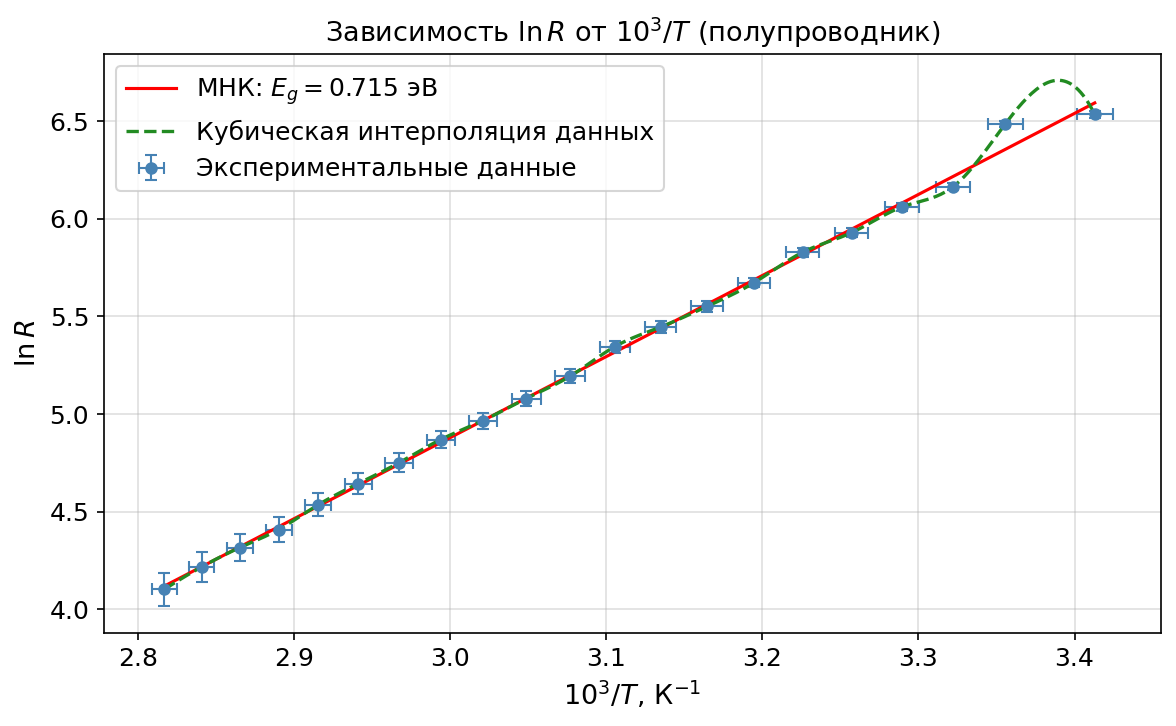
\includegraphics[width=0.88\textwidth]{plot_semiconductor}
    \caption{Зависимость $\ln R$ от $10^3/T$ для полупроводника. Точки — эксперимент (с погрешностями), прямая — МНК-аппроксимация.}
    \label{fig:semi}
\end{figure}

\subsection{График зависимости $R(t)$ (металл)}

По данным таблицы~\ref{tab:metal} построен график (рис.~\ref{fig:metal}).
Зависимость линейна, что подтверждает формулу~(\ref{eq:metal}).

\begin{figure}[H]
    \centering
    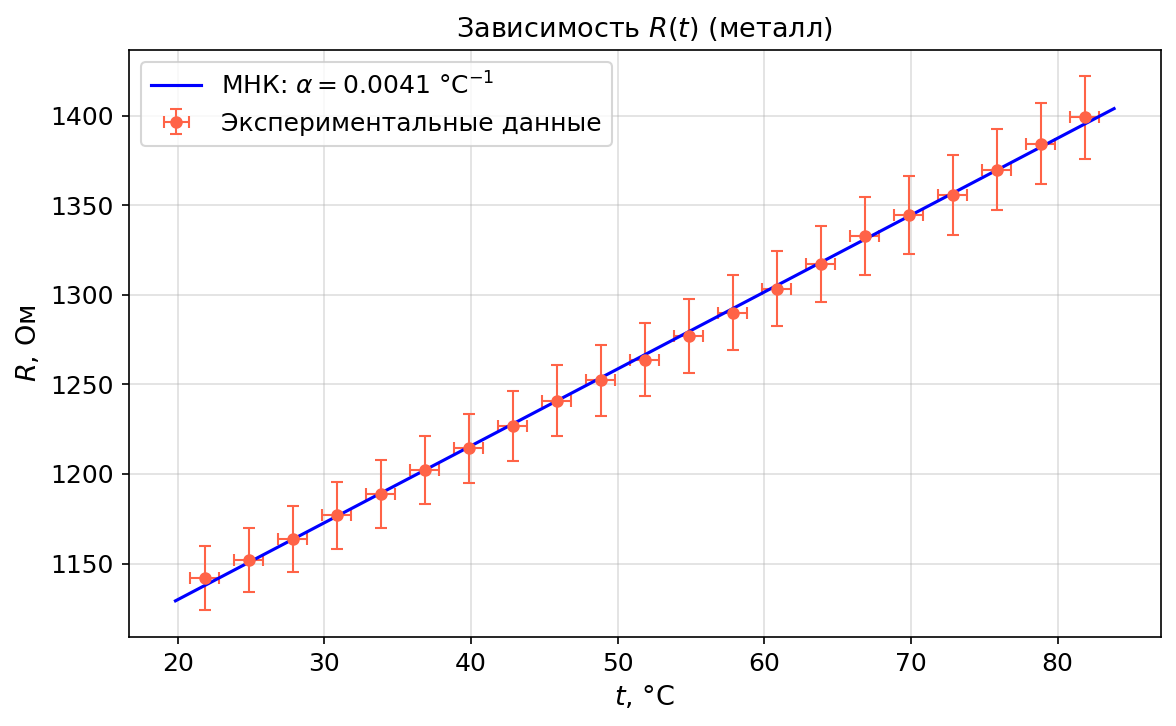
\includegraphics[width=0.88\textwidth]{plot_metal}
    \caption{Зависимость $R(t)$ для металла. Точки — эксперимент (с погрешностями), прямая — МНК-аппроксимация.}
    \label{fig:metal}
\end{figure}

% ===== ВЫЧИСЛЕНИЕ Eg МЕТОД ПАР =====
\subsection{Ширина запрещённой зоны полупроводника}

\subsubsection*{Метод пар}

Все 21 точку разбиваем на 10 независимых пар: точка $i$ объединяется с точкой $i+10$.
Для каждой пары по формуле~(\ref{eq:Eg_pair}) вычисляется $E_{g,ij}$.

\textbf{Пример расчёта} для пары $(1,\,11)$:
\[
    E_{g,1{-}11} = 2 \times 1{,}38065\times10^{-23}\,
    \frac{293 \cdot 325}{325 - 293}\,\ln\frac{688{,}16}{180{,}21}
    = 2k \cdot \frac{95225}{32} \cdot 1{,}3399
    \approx 1{,}101\times10^{-19}\ \text{Дж} = 0{,}687\ \text{эВ}.
\]

Результаты для всех пар сведены в таблицу~\ref{tab:eg_pairs}.

\begin{table}[H]
\centering
\caption{Результаты вычисления $E_g$ методом пар (полупроводник)}
\label{tab:eg_pairs}
\begin{tabular}{|c|c|c|c|}
\hline
Пара $(i,j)$ & $E_{g,ij}$, Дж & $E_{g,ij}$, эВ \\
\hline
(1, 11)  & $1{,}1010\times10^{-19}$ & 0.6872 \\
(2, 12)  & $1{,}2654\times10^{-19}$ & 0.7898 \\
(3, 13)  & $1{,}0978\times10^{-19}$ & 0.6852 \\
(4, 14)  & $1{,}1128\times10^{-19}$ & 0.6946 \\
(5, 15)  & $1{,}1219\times10^{-19}$ & 0.7003 \\
(6, 16)  & $1{,}1489\times10^{-19}$ & 0.7171 \\
(7, 17)  & $1{,}1249\times10^{-19}$ & 0.7021 \\
(8, 18)  & $1{,}1494\times10^{-19}$ & 0.7174 \\
(9, 19)  & $1{,}1572\times10^{-19}$ & 0.7223 \\
(10, 20) & $1{,}1765\times10^{-19}$ & 0.7343 \\
\hline
\end{tabular}
\end{table}

Среднее значение и случайная погрешность (доверительный интервал 95\%, $t_{0{,}95}(9) = 2{,}26$):
\[
    \langle E_g \rangle = \frac{1}{10}\sum_{k=1}^{10} E_{g,k}
    = 1{,}146\times10^{-19}\ \text{Дж} = 0{,}715\ \text{эВ},
\]
\[
    \sigma_{E_g} = 4{,}92\times10^{-21}\ \text{Дж} = 0{,}031\ \text{эВ},
\]
\[
    \Delta E_g = t_{0{,}95}\cdot\frac{\sigma_{E_g}}{\sqrt{n}}
    = 2{,}26 \cdot \frac{4{,}92\times10^{-21}}{\sqrt{10}}
    = 3{,}52\times10^{-21}\ \text{Дж} = 0{,}022\ \text{эВ}.
\]

\subsubsection*{Метод наименьших квадратов (МНК)}

По формуле~(\ref{eq:semi_lin}) МНК-аппроксимация даёт угловой коэффициент
$b = E_g/(2k)$:
\[
    b = 4150{,}8 \pm 46{,}4\ \text{К},
\]
\[
    E_g = 2k b = 2 \times 1{,}38065\times10^{-23} \times 4150{,}8
    = 1{,}146\times10^{-19}\ \text{Дж},
\]
\[
    \Delta E_g = 2k\,\Delta b = 2 \times 1{,}38065\times10^{-23} \times 46{,}4
    = 1{,}28\times10^{-21}\ \text{Дж}.
\]

\[
    \boxed{E_g\ \text{(МНК)} = (0{,}715 \pm 0{,}008)\ \text{эВ}}
\]

% ===== ВЫЧИСЛЕНИЕ АЛЬФА =====
\subsection{Температурный коэффициент сопротивления металла}

\subsubsection*{Метод пар}

Аналогично разбиваем 21 точку на 10 пар. Для каждой пары по формуле~(\ref{eq:alpha_pair}):

\textbf{Пример расчёта} для пары $(1,\,11)$:
\[
    \alpha_{1{-}11} = \frac{1141{,}84 - 1263{,}82}{1263{,}82 \cdot 21{,}85 - 1141{,}84 \cdot 51{,}85}
    = \frac{-121{,}98}{27614{,}5 - 59204{,}4}
    = \frac{-121{,}98}{-31589{,}9}
    \approx 3{,}861\times10^{-3}\ ^{\circ}\mathrm{C}^{-1}.
\]

Результаты для всех пар сведены в таблицу~\ref{tab:alpha_pairs}.

\begin{table}[H]
\centering
\caption{Результаты вычисления $\alpha$ методом пар (металл)}
\label{tab:alpha_pairs}
\begin{tabular}{|c|c|}
\hline
Пара $(i,j)$ & $\alpha_{ij}$, $10^{-3}\ ^{\circ}\mathrm{C}^{-1}$ \\
\hline
(1, 11)  & 3.861 \\
(2, 12)  & 3.969 \\
(3, 13)  & 4.027 \\
(4, 14)  & 4.030 \\
(5, 15)  & 4.091 \\
(6, 16)  & 4.183 \\
(7, 17)  & 4.167 \\
(8, 18)  & 4.115 \\
(9, 19)  & 4.115 \\
(10, 20) & 4.247 \\
\hline
\end{tabular}
\end{table}

Среднее значение и доверительный интервал (95\%, $t_{0{,}95}(9) = 2{,}26$):
\[
    \langle\alpha\rangle = \frac{1}{10}\sum_{k=1}^{10}\alpha_k
    = 4{,}0804\times10^{-3}\ ^{\circ}\mathrm{C}^{-1},
\]
\[
    \sigma_\alpha = 1{,}126\times10^{-4}\ ^{\circ}\mathrm{C}^{-1},
    \qquad
    \Delta\alpha = 2{,}26 \cdot \frac{1{,}126\times10^{-4}}{\sqrt{10}}
    = 8{,}05\times10^{-5}\ ^{\circ}\mathrm{C}^{-1}.
\]

\[
    \boxed{\alpha\ \text{(метод пар)} = (4{,}080 \pm 0{,}081)\times10^{-3}\ ^{\circ}\mathrm{C}^{-1}}
\]

\subsubsection*{Метод наименьших квадратов (МНК)}

Аппроксимация $R(t) = R_0 + S\cdot t$ даёт:
\[
    R_0 = 1044{,}04\ \text{Ом}, \qquad S = 4{,}2915\ \text{Ом}/^{\circ}\mathrm{C},
\]
\[
    \alpha = \frac{S}{R_0} = \frac{4{,}2915}{1044{,}04} = 4{,}110\times10^{-3}\ ^{\circ}\mathrm{C}^{-1}.
\]

\[
    \boxed{\alpha\ \text{(МНК)} = 4{,}110\times10^{-3}\ ^{\circ}\mathrm{C}^{-1}}
\]

% ===== ИТОГОВЫЕ РЕЗУЛЬТАТЫ =====
\section{Итоговые результаты и погрешности}

\begin{table}[H]
\centering
\caption{Сводная таблица результатов}
\label{tab:results}
\begin{tabular}{|l|c|c|}
\hline
\textbf{Величина} & \textbf{Метод пар} & \textbf{МНК} \\
\hline
$E_g$, эВ & $0{,}715 \pm 0{,}022$ & $0{,}715 \pm 0{,}008$ \\
$E_g$, Дж & $(1{,}146 \pm 0{,}035)\times10^{-19}$ & $(1{,}146 \pm 0{,}013)\times10^{-19}$ \\
$\alpha$, $10^{-3}\ ^{\circ}\mathrm{C}^{-1}$ & $4{,}080 \pm 0{,}081$ & $4{,}110$ \\
\hline
\end{tabular}
\end{table}

Оба метода дают согласующиеся результаты. МНК обеспечивает меньшую погрешность, так как задействует все точки одновременно.

% ===== ИДЕНТИФИКАЦИЯ =====
\section{Идентификация образцов}

\subsection*{Полупроводник}

Полученное значение ширины запрещённой зоны:
\[
    E_g = (0{,}715 \pm 0{,}022)\ \text{эВ}.
\]

Сравнение со справочными данными:

\begin{table}[H]
\centering
\begin{tabular}{|l|c|}
\hline
\textbf{Материал} & $E_g$, эВ \\
\hline
Германий (Ge) & 0.67 \\
Кремний (Si)  & 1.12 \\
\hline
\end{tabular}
\end{table}

Измеренное значение $E_g \approx 0{,}715$\,эВ наиболее близко к табличному значению для \textbf{германия} ($E_g^\text{табл} = 0{,}67$\,эВ). Расхождение составляет $\approx 7\%$, что может быть обусловлено примесной проводимостью образца, нагревом при измерении тока и погрешностью приборов.

\subsection*{Металл}

Полученное значение ТКС:
\[
    \alpha = (4{,}08 \pm 0{,}08)\times10^{-3}\ ^{\circ}\mathrm{C}^{-1}.
\]

Сравнение со справочными данными:

\begin{table}[H]
\centering
\begin{tabular}{|l|c|}
\hline
\textbf{Материал} & $\alpha$, $10^{-3}\ ^{\circ}\mathrm{C}^{-1}$ \\
\hline
Медь (Cu)      & 4.3 \\
Алюминий (Al)  & 4.0 \\
Вольфрам (W)   & 4.5 \\
Никель (Ni)    & 6.0 \\
Платина (Pt)   & 3.9 \\
\hline
\end{tabular}
\end{table}

Значение $\alpha \approx 4{,}08\times10^{-3}\ ^{\circ}\mathrm{C}^{-1}$ хорошо совпадает со справочными данными для \textbf{алюминия} ($\alpha^\text{табл} = 4{,}0\times10^{-3}\ ^{\circ}\mathrm{C}^{-1}$, расхождение $\approx 2\%$) и для \textbf{платины} ($\alpha^\text{табл} = 3{,}9\times10^{-3}\ ^{\circ}\mathrm{C}^{-1}$). Наиболее вероятный материал — \textbf{алюминий} или \textbf{платина}.

% ===== ВЫВОДЫ =====
\section{Выводы}

\begin{enumerate}
    \item Экспериментально получены зависимости $R(T)$ металлического и полупроводникового образцов в диапазоне температур $\approx 295$–$355$\,К.

    \item Для металла зависимость $R(t)$ линейна, как и предсказывает теория. Методом пар и МНК определён температурный коэффициент сопротивления:
    \[
        \alpha = (4{,}08 \pm 0{,}08)\times10^{-3}\ ^{\circ}\mathrm{C}^{-1}.
    \]
    По этому значению образец идентифицируется как \textbf{алюминий} (или платина).

    \item Для полупроводника зависимость $\ln R$ от $1/T$ линейна, что подтверждает экспоненциальный характер зависимости $R(T)$. Ширина запрещённой зоны:
    \[
        E_g = (0{,}715 \pm 0{,}008)\ \text{эВ} \quad \text{(МНК)}.
    \]
    Результат соответствует \textbf{германию} ($E_g^\text{табл} = 0{,}67$\,эВ).

    \item Оба метода обработки (метод пар и МНК) дают согласующиеся результаты; МНК обеспечивает меньшую погрешность.
\end{enumerate}

\end{document}

